% arara: xelatex: { shell: yes }
% arara: biber
% arara: nomencl
% arara: xelatex: { shell: yes }
% arara: xelatex: { shell: yes }
\documentclass[nolibertine, ngerman]{ttlab-qualify}
% mögliche Optionen:
% - ngerman
% - english
% - minted
% - algorithm
% - nomencl
% - nolibertine
\usepackage{libertine}
\usepackage{hyperref}
\hypersetup{
    colorlinks=true,      % Aktiviert farbige Links
    urlcolor=blue,        % URLs in Blau
    linkcolor=black,      % Interne Links (z.B. Abschnittsverweise) in Schwarz
    citecolor=black,      % Zitatverweise (Bibliographie) in Schwarz
    filecolor=black,      % Dateilinks in Schwarz
    menucolor=black       % Acrobat-Menülinks in Schwarz
}
\urlstyle{same}

\addbibresource{bib.bib}

\begin{document}

\titlehead{
  Kenan Khauto\\
  7592047\\
  B.Sc Informatik\\
  Studienfachkombination / Schwerpunkt \\
  6\\
  kenan.khauto@stud.uni-frankfurt.de 
}
\subject{Seminararbeit Text Analytics}
\author{Kenan Khauto}
\title{Image Understanding}
\subtitle{Lernen visueller Konzepte beim Inferieren ohne finetuning}
\date{Abgabedatum: <Datum>}
\publishers{Goethe-Universität Frankfurt am Main\\Prof. Alexander Mehler}

\maketitle


\tableofcontents

\chapter{Einleitung}
Im Bereich der künstlichen Intelligenz und des maschinellen Lernens hat sich in den letzten Jahren eine bemerkenswerte Entwicklung 
vollzogen, insbesondere im Verständnis visueller Konzepte durch Modelle wie CLIP (Contrastive Language–Image Pretraining). 
Diese Modelle haben das traditionelle Paradigma, das umfangreiche Fine-Tuning und spezialisierte Datensätze erforderte, herausgefordert 
und bieten neue Wege, wie Maschinen Bilder und Texte in einem zusammenhängenden Rahmen verstehen können.


Die Kernfrage, die wir in diesem Seminar untersuchen, lautet: "Wie können KI-Modelle wie CLIP visuelle Konzepte effektiv durch 
Inferenz verstehen und interpretieren, ohne dass ein umfangreiches Fine-Tuning erforderlich ist?" Diese Frage berührt die Grundlagen 
der Art und Weise, wie maschinelle Lernmodelle trainiert und angewendet werden, insbesondere im Kontext der Integration von visuellen und 
textuellen Daten.


CLIP, ein Produkt von OpenAI, repräsentiert einen Durchbruch in der Art und Weise, wie Maschinen lernen, Bilder und Texte zu verbinden. 
Anstatt sich auf umfangreiche, spezialisierte Datensätze zu verlassen, nutzt CLIP ein breites Spektrum an Internetdaten und lernt, 
visuelle Konzepte direkt aus einer Vielzahl von Bildern und den dazugehörigen Beschreibungen zu extrahieren. Dieser Ansatz ermöglicht 
es dem Modell, eine breite Palette von visuellen Konzepten zu verstehen, ohne für jedes neue Konzept speziell angepasst zu werden.


In diesem Seminar werden wir die Mechanismen hinter CLIP und ähnlichen Modellen erforschen. Wir werden untersuchen, wie diese Modelle 
trainiert werden, ihre Fähigkeit, visuelle Daten zu interpretieren, und die Herausforderungen, denen sie gegenüberstehen, wie zum Beispiel 
die Behandlung von Verzerrungen und die Generalisierbarkeit ihrer Erkenntnisse. Darüber hinaus werden wir diskutieren, wie diese Technologien 
in verschiedenen Anwendungsfeldern eingesetzt werden könnten, von der automatisierten Bildbeschreibung bis hin zur Verbesserung 
der Mensch-Maschine-Interaktion.

\chapter{Hauptteil}
\section{Theoretischer Hintergrund}
Dieser Abschnitt stellt die theoretischen Grundlagen vor, die für das Verständnis der Funktionsweise von KI-Modellen wie CLIP (Contrastive Language–Image Pretraining) essentiell sind. Hier werden die Kernelemente des maschinellen Lernens, die Besonderheiten des Deep Learning und die Bedeutung des kontrastiven Lernens für die Verarbeitung von Bild- und Textdaten erörtert.

\subsection{Grundlagen des maschinellen Lernens}

Maschinelles Lernen ist ein Teilgebiet der künstlichen Intelligenz, das sich mit der Entwicklung von Algorithmen beschäftigt, die Computern das Lernen aus Daten ermöglichen. Die Hauptzielsetzung des maschinellen Lernens ist es, Muster in Daten zu erkennen und auf Basis dieser Muster Vorhersagen oder Entscheidungen zu treffen.

\textbf{Überwachtes vs. unüberwachtes Lernen:} Überwachtes Lernen bezieht sich auf Lernprozesse, bei denen das Modell anhand von Beispieldaten und bekannten Ausgabewerten trainiert wird. Unüberwachtes Lernen hingegen befasst sich mit dem Finden von Mustern oder Strukturen in Daten, ohne vorherige Kenntnis der Ausgabewerte.

\textbf{Verstärkendes Lernen:} Eine weitere wichtige Lernmethode ist das verstärkende Lernen, bei dem ein Modell durch Belohnungen lernt, bestimmte Aktionen in einer Umgebung auszuführen, um ein bestimmtes Ziel zu erreichen.

\subsection{Deep Learning und neuronale Netzwerke}

Deep Learning, eine Unterklasse des maschinellen Lernens, basiert auf künstlichen neuronalen Netzwerken mit vielen Schichten (sogenannten "tiefen" Netzwerken). Diese Netzwerke sind in der Lage, komplexe Muster in großen Datenmengen zu erkennen.

\begin{figure}[h]
	\centering
	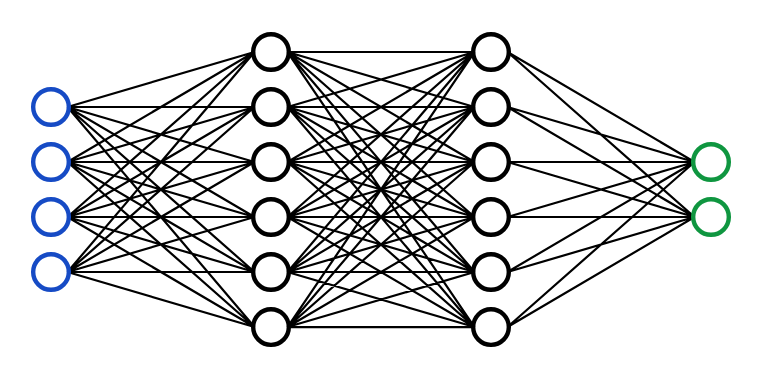
\includegraphics[scale=0.4]{static/FCnetwork.png}
	\caption{A simple fully connected neural network, see \url{https://victorzhou.com/series/neural-networks-from-scratch/}}
	\label{fig:2.1}
\end{figure}

\textbf{Convolutional Neural Networks (CNNs):} Speziell für die Bildverarbeitung sind CNNs von entscheidender Bedeutung. Sie sind darauf ausgelegt, hierarchische Muster in Bildern zu erkennen, was sie ideal für Aufgaben wie Bildklassifikation und Objekterkennung macht.
\begin{figure}[h]
	\centering
	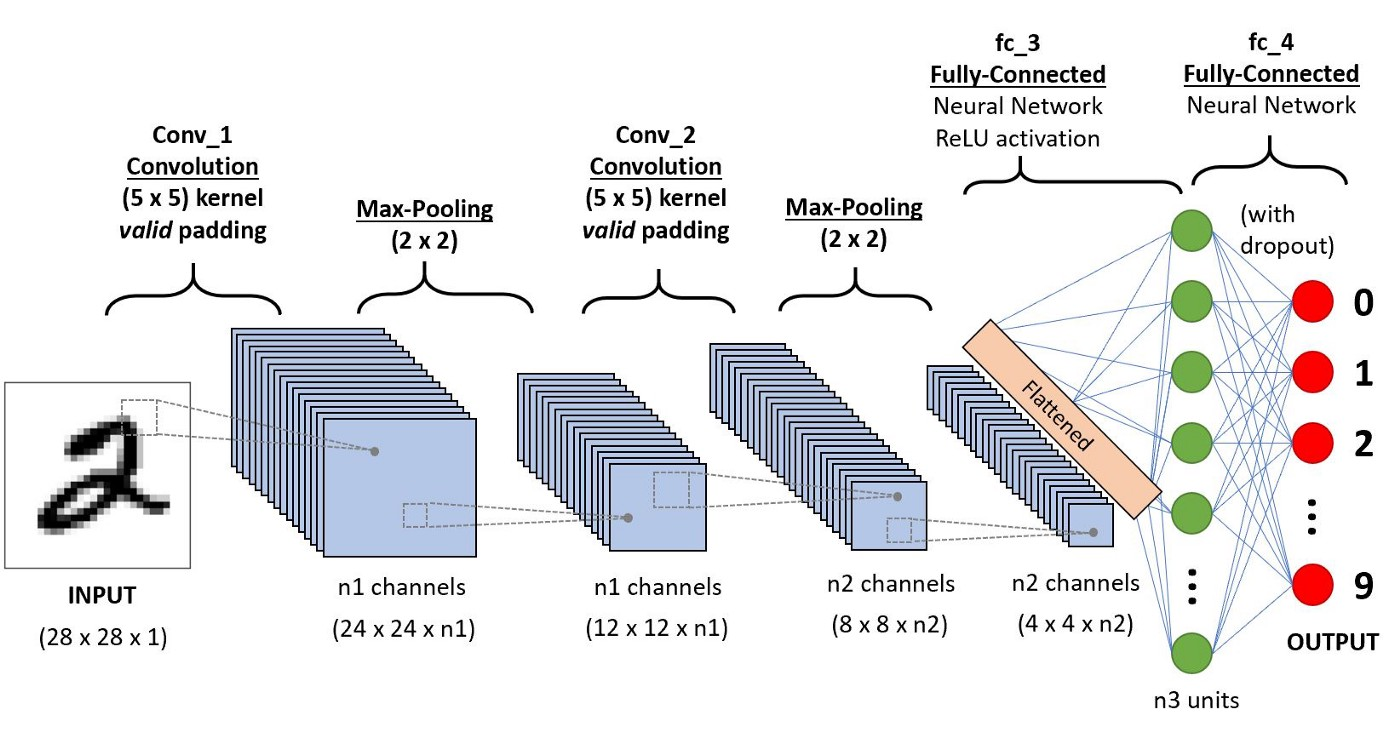
\includegraphics[scale=0.2]{static/cnn.jpeg}
	\caption{Convolutional neural network (CNN), see \url{https://paperswithcode.com/methods/category/convolutional-neural-networks}}
	\label{fig:2.2}
\end{figure}

\textbf{Transformer-Modelle:} Ursprünglich in der Verarbeitung natürlicher Sprache eingesetzt, haben Transformer-Modelle aufgrund ihrer Fähigkeit, langfristige Abhängigkeiten in Daten zu erkennen, zunehmend Anwendung in anderen Bereichen, einschließlich der Bildverarbeitung, gefunden.
\begin{figure}[h]
	\centering
	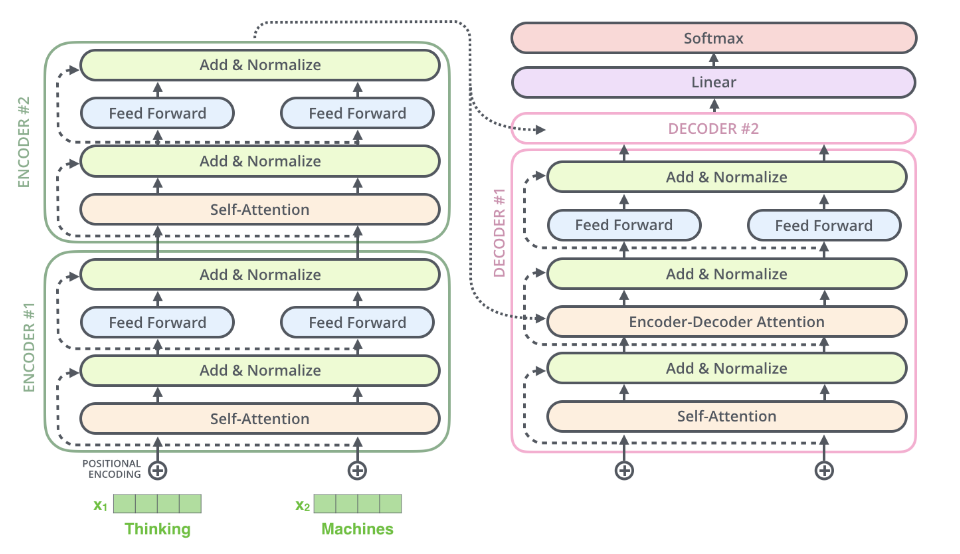
\includegraphics[scale=0.5]{static/transformer.png}
	\caption{Transformer with two encoders, 2 decoders and a fully connected layer for prediction, see \url{http://jalammar.github.io/illustrated-transformer/}}
	\label{fig:2.3}
\end{figure}

\subsection{Kontrastives Lernen und CLIP}
Kontrastives Lernen ist eine Technik, die darauf abzielt, ähnliche Datenpunkte näher zusammenzubringen und unähnliche weiter voneinander zu entfernen. CLIP verwendet kontrastives Lernen, um die Beziehungen zwischen Bildern und Text zu verstehen.

\textbf{Funktionsweise von CLIP:} CLIP wird mit einer Vielzahl von Bildern und den dazugehörigen Textbeschreibungen trainiert. Das Modell lernt, die Verbindungen zwischen Bildern und Texten zu verstehen, was es ihm ermöglicht, eine breite Palette von Bildinhalten effektiv zu interpretieren.

\textbf{Vorteile gegenüber traditionellen Ansätzen:} Im Gegensatz zu traditionellen Bilderkennungsmodellen, die oft umfangreiches Fine-Tuning für spezifische Aufgaben benötigen, kann CLIP vielfältige visuelle Konzepte anhand seiner Trainingsdaten erkennen und interpretieren, was eine größere Flexibilität und Anpassungsfähigkeit bedeutet.
\section{Analyse von CLIP und ähnlichen Modellen}
\section{Fallstudien / Anwendungen}
Hier erwähnen wo und wie CLIP in image understanding paper benutzt wurde.
\section{Diskussion von Herausforderungen und Grenzen}
\section{Zukünftige Richtungen und mögliche Verbesserungen}

\printbibliography
\appendix

\end{document}
